% Options for packages loaded elsewhere
\PassOptionsToPackage{unicode}{hyperref}
\PassOptionsToPackage{hyphens}{url}
%
\documentclass[
  10pt,
]{article}
\usepackage{amsmath,amssymb}
\usepackage{lmodern}
\usepackage{iftex}
\ifPDFTeX
  \usepackage[T1]{fontenc}
  \usepackage[utf8]{inputenc}
  \usepackage{textcomp} % provide euro and other symbols
\else % if luatex or xetex
  \usepackage{unicode-math}
  \defaultfontfeatures{Scale=MatchLowercase}
  \defaultfontfeatures[\rmfamily]{Ligatures=TeX,Scale=1}
\fi
% Use upquote if available, for straight quotes in verbatim environments
\IfFileExists{upquote.sty}{\usepackage{upquote}}{}
\IfFileExists{microtype.sty}{% use microtype if available
  \usepackage[]{microtype}
  \UseMicrotypeSet[protrusion]{basicmath} % disable protrusion for tt fonts
}{}
\makeatletter
\@ifundefined{KOMAClassName}{% if non-KOMA class
  \IfFileExists{parskip.sty}{%
    \usepackage{parskip}
  }{% else
    \setlength{\parindent}{0pt}
    \setlength{\parskip}{6pt plus 2pt minus 1pt}}
}{% if KOMA class
  \KOMAoptions{parskip=half}}
\makeatother
\usepackage{xcolor}
\IfFileExists{xurl.sty}{\usepackage{xurl}}{} % add URL line breaks if available
\IfFileExists{bookmark.sty}{\usepackage{bookmark}}{\usepackage{hyperref}}
\hypersetup{
  pdftitle={Analisis de Trafico y modelo predictivo para la detección de eventos maliciosos en Equipos IOT},
  pdfauthor={Grupo1 (Rosa Valencia - Ydael Vargas - Elizabeth Longa)},
  hidelinks,
  pdfcreator={LaTeX via pandoc}}
\urlstyle{same} % disable monospaced font for URLs
\usepackage[margin=1in]{geometry}
\usepackage{graphicx}
\makeatletter
\def\maxwidth{\ifdim\Gin@nat@width>\linewidth\linewidth\else\Gin@nat@width\fi}
\def\maxheight{\ifdim\Gin@nat@height>\textheight\textheight\else\Gin@nat@height\fi}
\makeatother
% Scale images if necessary, so that they will not overflow the page
% margins by default, and it is still possible to overwrite the defaults
% using explicit options in \includegraphics[width, height, ...]{}
\setkeys{Gin}{width=\maxwidth,height=\maxheight,keepaspectratio}
% Set default figure placement to htbp
\makeatletter
\def\fps@figure{htbp}
\makeatother
\setlength{\emergencystretch}{3em} % prevent overfull lines
\providecommand{\tightlist}{%
  \setlength{\itemsep}{0pt}\setlength{\parskip}{0pt}}
\setcounter{secnumdepth}{-\maxdimen} % remove section numbering
\ifLuaTeX
  \usepackage{selnolig}  % disable illegal ligatures
\fi

\title{Analisis de Trafico y modelo predictivo para la detección de
eventos maliciosos en Equipos IOT}
\author{Grupo1 (Rosa Valencia - Ydael Vargas - Elizabeth Longa)}
\date{Fecha: 2022-05-29}

\begin{document}
\maketitle

\hypertarget{introducciuxf3n}{%
\subsection{\texorpdfstring{\textbf{INTRODUCCIÓN}}{INTRODUCCIÓN}}\label{introducciuxf3n}}

Internet de las cosas (IoT) es una de las tecnologías líderes en la
actualidad y se considera una extensión natural de Internet al
incorporar sensores y comunicaciones de máquina a máquina. Las
aplicaciones de IoT han aparecido en una variedad de dominios que
incluyen atención médica, estado físico, administración de energía en el
hogar, automatización de aulas, ciudades inteligentes y muchos más. Una
aplicación típica de IoT consta de tres capas; la capa de percepción, la
capa de red y la capa de aplicación. La capa de percepción es
responsable de detectar y recopilar información sobre el entorno y
enviarla a la capa de red. Por ejemplo, las cámaras de vigilancia son un
tipo de sensor que reconoce eventos inusuales como el movimiento
mediante sensores. La capa de red/transporte se considera un vínculo
entre la capa de percepción y la nube. Esta capa consta de muchos
protocolos de Internet y tiene que integrar la comunicación.

IoT es vulnerable a los riesgos de seguridad en cada capa arquitectónica
y ha enfrentado desafíos de seguridad desde su aparición. Los
dispositivos IoT requieren sistemas de autenticación sólidos, que muchos
dispositivos IoT no tienen debido a limitaciones de recursos como CPU o
limitaciones de energía/batería. La capa de aplicación también está
abierta a ataques de virus, gusanos y ataques de phishing.

Uno de los métodos clave para prevenir este tipo de ataques es el
despliegue de un sistema de detección de intrusos (IDS) sólido que pueda
detectar cualquier tipo de intrusión. Actualmente, los IDS utilizan dos
métodos principales para detectar ataques: basados en firmas y basados
en anomalías. Los métodos basados en firmas dependen de los ataques
conocidos y sus actualizaciones requieren mucho tiempo. Los ataques
basados en anomalías, por otro lado, se basan en datos y dependen de que
la máquina comprenda el comportamiento normal y rechace

\hypertarget{metodologuxeda}{%
\subsection{\texorpdfstring{\textbf{METODOLOGÍA}}{METODOLOGÍA}}\label{metodologuxeda}}

Este documento utilizó el conjunto de datos IoT-23
(CTU-IoT-Malware-Capture-1-1) archivo \textbf{conn.log.labeled}
{[}\url{https://www.stratosphereips.org/datasets-iot23}{]}. Estos datos
se basan en el tráfico de red obtenido de dispositivos de Internet de
las cosas (IoT) conregistros queevidencian detección de malware y
capturas benignas.

Para el presente analisis se han considerado los siguientes pasos:

\begin{verbatim}
- Identificación de las variables
- Tratamiento de datos perdidos
- Tratamiento de outliers
- Transformación de variables
- Creación de variables dummy
- Identificación de variables con variancia cero o casi cero
- Identificación de predictores correlacionados
\end{verbatim}

\hypertarget{identificaciuxf3n-de-las-variables}{%
\subsubsection{\texorpdfstring{\textbf{Identificación de las
variables}}{Identificación de las variables}}\label{identificaciuxf3n-de-las-variables}}

A continuación se procede con la exploración de datos con la finalidad
deidentificar nuestras variables representativas, para estefin leemos
los datos de nuestro dataset.

\begin{figure}
\centering
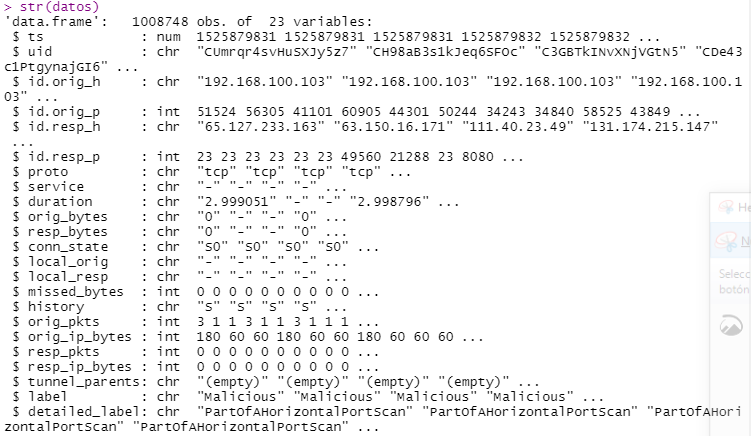
\includegraphics{Resumen_Estructura_Datos.PNG}
\caption{\textbf{Estructura de Datos}}
\end{figure}

\hypertarget{tratamiento-de-datos-perdidos}{%
\subsubsection{\texorpdfstring{\textbf{Tratamiento de datos
perdidos}}{Tratamiento de datos perdidos}}\label{tratamiento-de-datos-perdidos}}

\hypertarget{tratamiento-de-outliers}{%
\subsubsection{\texorpdfstring{\textbf{Tratamiento de
outliers}}{Tratamiento de outliers}}\label{tratamiento-de-outliers}}

\hypertarget{transformaciuxf3n-de-variables}{%
\subsubsection{\texorpdfstring{\textbf{Transformación de
variables}}{Transformación de variables}}\label{transformaciuxf3n-de-variables}}

\hypertarget{creaciuxf3n-de-variables-dummy}{%
\subsubsection{\texorpdfstring{\textbf{Creación de variables
dummy}}{Creación de variables dummy}}\label{creaciuxf3n-de-variables-dummy}}

\hypertarget{identificaciuxf3n-de-variables-con-variancia-cero-o-casi-cero}{%
\subsubsection{\texorpdfstring{\textbf{Identificación de variables con
variancia cero o casi
cero}}{Identificación de variables con variancia cero o casi cero}}\label{identificaciuxf3n-de-variables-con-variancia-cero-o-casi-cero}}

\hypertarget{identificaciuxf3n-de-predictores-correlacionados}{%
\subsubsection{\texorpdfstring{\textbf{Identificación de predictores
correlacionados}}{Identificación de predictores correlacionados}}\label{identificaciuxf3n-de-predictores-correlacionados}}

\end{document}
